
% =========================================================
\section{Introduction}
\begin{frame}
	\frametitle{Introduction}
	\framesubtitle{Business Understanding - Legislative Proposal's Definition and Types}

	\begin{exampleblock}{Legislative Proposal} 
	\begin{itemize}
		\item A \textbf{Legislative Proposal} is any matter subject to deliberation by the Legislative Chamber (CLDF Internal Regulations, art. 129).
	\end{itemize}
	\end{exampleblock}

	% Introdução: Entendendo o Negócio

	% Uma proposição legislativa é toda matéria sujeita à deliberação na Câmara Legislativa.
	% Elas incluem (ler cada uma).


	\begin{exampleblock}{} 
	\textbf{Legislative Proposals can be of the following types:}
	\begin{multicols}{2}
		\begin{itemize}
			\item Proposta de emenda à Lei Orgânica;
			
			\item Projeto de lei complementar;
			
			\item Projeto de lei;
			
			\item Projeto de decreto legislativo;
			
			\item Projeto de resolução;
			
			\item Indicação;
			
			\item Moção;
			
			\item Requerimento;
			
			\item Emenda;
			
			\item Recursos;
		\end{itemize}
	\end{multicols}
	\end{exampleblock}
\end{frame}
% --------------------------------------------------------------------------------------------
\begin{frame}
	\frametitle{Introduction}
	\framesubtitle{Business Understanding - Legislative Proposal's Themes}

	% As proposições são classificadas em um ou mais temas, dentro de um total de 34 temas disponíveis.
	
	% Por exemplo, uma mesma proposição pode ser classificada como: Assunto Social, Saúde e Educação.  
	% Por exemplo, uma mesma proposição pode ser classificada como: Assunto Social, Saúde e Educação.  


	%https://ple.cl.df.gov.br/#/proposicao/buscar	
	\begin{exampleblock}{Legislative Proposals are classified into one or more themes:} 
		\begin{multicols}{3}
			\begin{itemize}
				\scriptsize
				\item Agricultura
				\item Assistência Social
				\item Assunto Fundiário e Ordenamento Territorial
				\item Assunto Social
				\item Cidadania
				\item Ciência e Tecnologia
				\item Combate à Corrupção
				\item Comunicação
				\item Comércio e Serviços
				\item Cultura
				\item Defesa do Consumidor
				\item Desenvolvimento Econômico
				\item Desporto e Lazer
				\item Direitos Humanos
				\item Economia
				\item Educação
				\item Energia
				\item Fiscalização e Governança
				\item Habitação
				\item Incentivos Fiscais e Concessões Públicas
				\item Indústria
				\item Meio Ambiente
				\item Não se aplica
				\item Outro
				\item Previdência Social
				\item Relações Exteriores
				\item Saneamento
				\item Saúde
				\item Segurança
				\item Servidor Público
				\item Trabalho
				\item Transporte e Mobilidade Urbana
				\item Turismo
				\item Urbanismo
				\normalsize
			\end{itemize}
		\end{multicols}
		\textbf{Total:} 34 themes	
	\end{exampleblock}
\end{frame}
% --------------------------------------------------------------------------------------------
\begin{frame}
	\frametitle{Introduction}
	\framesubtitle{Business Understanding - Why Themes?}
	\begin{block}{Thematic Classification Benefits} % Block without title
		\begin{itemize}
			\item Efficient classification of legislative proposals is crucial to \textbf{streamline their analysis} and processing within the legislative process helping to \textbf{determine which committees a proposal should go through}.
					
			% Existem diversas razões para realizar essa classificação. 
							
			% Uma classificação eficiente ajuda a otimizar a análise e o processamento dentro do processo legislativo, ajudando a determinar em quais comissões uma proposta deve passar.

			\item By categorizing legislative proposals into relevant themes, lawmakers can streamline their analysis, \textbf{allocate resources efficiently}, and \textbf{make informed decisions}. 

			% Ajuda os legisladores a alocar recursos de forma eficiente e a tomar decisões informadas.

			\item This process \textbf{enhances transparency} and facilitates a more \textbf{organized legislative workflow}.	
			% Melhora a transparência e facilita um fluxo legislativo mais organizado.

					
			\item Thematic classification plays an important role in maintaining \textbf{accurate information retrieval} and \textbf{ensuring effective legislative management}.
			
			% Em resumo, a classificação temática desempenha um papel importante na manutenção da recuperação precisa de informações e na garantia de uma gestão legislativa eficaz.
				
		\end{itemize}
	\end{block}
\end{frame}
% =========================================================
\section{The Problem}
\begin{frame}
	\frametitle{The Problem}
	\framesubtitle{Understanding the problem}
	
	% Qual é o problema?
	
	\begin{alertblock}{Theme ``others'' is growing bigger}
		\begin{itemize}
			\item 	Usually, the author of the proposal is responsible for classifying it into one or more themes.
			
			% A escolha dos temas para classificar uma proposição é geralmente feita pelo autor da proposição.
			
			\item Unfortunately, due to various factors such as ambiguous topics, outdated categories, multidisciplinary nature, \textbf{many propositions end up being classified under the generic label of ``others''}.
			
			% Contudo, infelizmente, devido a diversos fatores, como tópicos ambíguos, categorias desatualizadas e natureza multidisciplinar, muitas proposições acabam sendo classificadas sob o rótulo genérico de “outros”.
			
		\end{itemize}
	\end{alertblock}	
\end{frame}
% --------------------------------------------------------------------------------------------
\begin{frame}
	\frametitle{The Problem}
	\framesubtitle{Understanding the problem}	
	\begin{figure}
		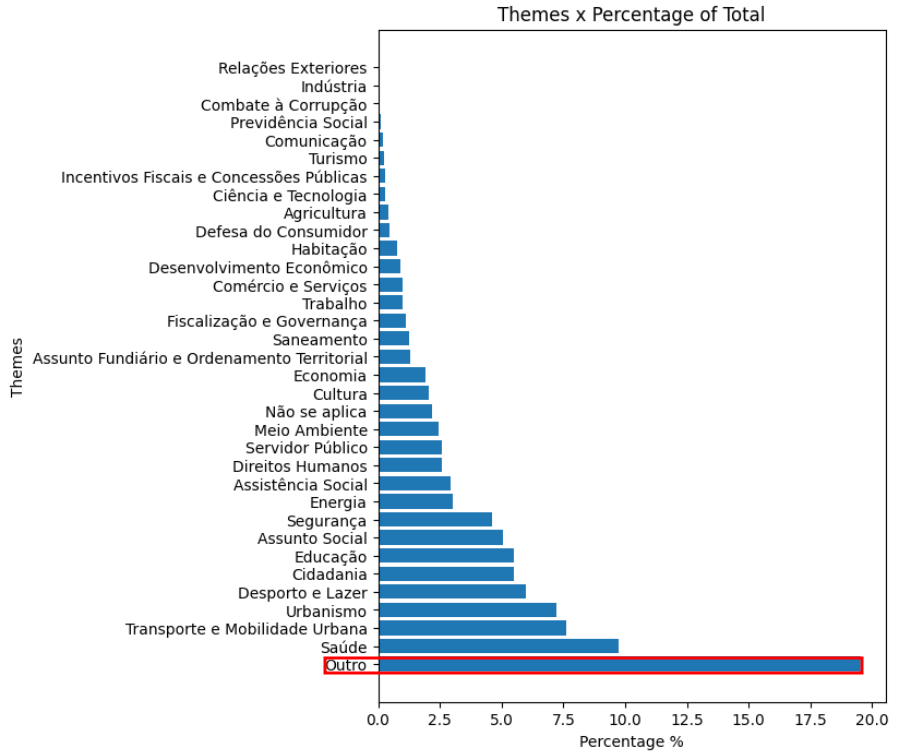
\includegraphics[width=0.6\linewidth]{graphThemes.png}
	\end{figure}

	% Para ilustrar esse problema, nesse gráfico mostramos o percentual do total de proposições classificadas em cada tema até maio de 2024.

	\begin{block}{}
		\scriptsize
		The chart shows that the number of proposals classified under the theme “others” represents approximately 20\% of the total. 
	\end{block}	

	% O gráfico mostra que o número de proposições classificadas com o tema "outros" já corresponde a quase 20% do total.

\end{frame}
% --------------------------------------------------------------------------------------------
\begin{frame}
	\frametitle{The Problem}
	\framesubtitle{Problem definition}	

	\begin{alertblock}{The problem is inadequate proposal classification}
		Inadequate classification hinders efficient tracking, analysis, and transparency of legislative activities, making it difficult for both society and lawmakers to understand and oversee the legislative process effectively.
	\end{alertblock}	

	\begin{figure}
		
\includegraphics[width=0.3\linewidth]{problem.jpeg}
	\end{figure}

	% O problema, portanto, é a classificação inadequada de proposições sobre o tema "outros".

	% Essa classificação inadequada dificulta o acompanhamento eficiente, a análise e a transparência das atividades legislativas, tornando desafiador tanto para a sociedade quanto para os legisladores compreender e supervisionar efetivamente o processo legislativo. 
\end{frame}
% =========================================================
\section{Objective}

\begin{frame}
	\frametitle{Objectives}
	\framesubtitle{Primary objective}
	
	\begin{exampleblock}{Primary objective} 
		\begin{itemize}
			\item The primary objective of this study is to \textbf{compare different machine learning models} to determine which model is \textbf{most effective in suggesting more appropriate theme categories for legislative proposals}.
			
			\item The goal is to find \textbf{more suitable themes that better match the content of these proposals}.  
		\end{itemize}
	\end{exampleblock}
	
	\begin{figure}
		
\includegraphics[width=0.3\linewidth]{arrow.jpeg}
	\end{figure}
	
	
\end{frame}


\begin{frame}
	\frametitle{Objectives}
	\framesubtitle{Disclaimer}
		
	\begin{alertblock}{Atention!} 
		\begin{itemize}
			\item This study \textbf{does not aim to automate the classification process, replace human classification, or compare human classification with machine learning classification}. 
			
			\item Instead, \textbf{the focus is on enhancing the existing categorization process by identifying the best model for suggesting themes for proposals currently classified under the generic label "others."}.
		\end{itemize}
	\end{alertblock}
	
	
	
\end{frame}

% ----------------------




% =========================================================
\section{Literature review}
\begin{frame}
	\frametitle{Literature review}
	
	\begin{thebibliography}{99} % Beamer does not support BibTeX so references must be inserted manually as below, you may need to use multiple columns and/or reduce the font size further if you have many references
	\footnotesize % Reduce the font size in the bibliography
		\scriptsize
	
		\bibitem[Reimers, 2019]{p1}
		Reimers, Nils and Gurevych, Iryna (2019)
		\newblock \href{http://arxiv.org/abs/1908.10084}{Sentence-BERT: Sentence Embeddings using Siamese BERT-Networks}
		\newblock \emph{Proceedings of the 2019 Conference on Empirical Methods in Natural Language Processing} 
		\newblock \emph{Association for Computational Linguistics} 
		
		\bibitem[Junior, 2021]{p2}
		J. Andrade Junior, J. Cardoso-Silva, and L. Bezerra (2021)
		\newblock \href{https://core.ac.uk/download/491169432.pdf}{Comparing Contextual Embeddings for	Semantic Textual Similarity in Portuguese}
		\newblock \scriptsize \emph{Anais da X Brazilian Conference on Intelligent Systems} 
		
		\normalsize		 

	\end{thebibliography}

	
	
\end{frame}
% =========================================================
\section{Methodology}

\begin{frame}
	\frametitle{Methodology}
	\framesubtitle{CRISP-DM's Methodology}	
	% Utilizamos a metodologia CRISP-DM.	
	\begin{figure}
		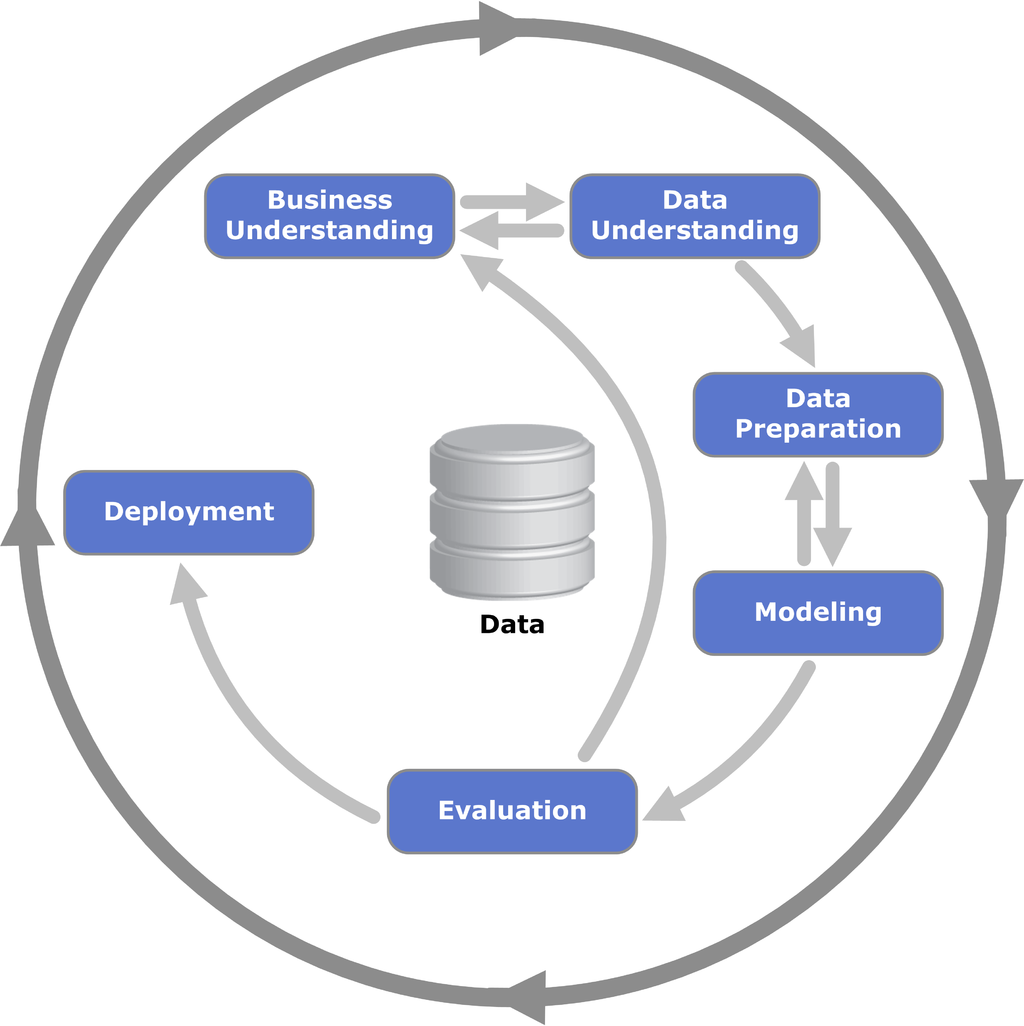
\includegraphics[width=0.5\linewidth]{crispdm.png}
	\end{figure}

	\begin{block}{}
	\scriptsize
		We utilized the CRISP-DM methodology. Its stages will be explained in the following slides.	
	\end{block}	
\end{frame}

% --------------------------------------------------------
\begin{frame}
	\frametitle{Methodology}
	\framesubtitle{1 - Business Understanding}	
	
	\begin{block}{1 - Business Understanding} 
			We have analyzed legislative documents to align our data mining objectives with legislative classification needs.
	\end{block}

	% Na primeira etapa do CRISP-DM "Entendimento do Negócio", nós analisamos diversos documentos para alinhar nossos objetivos de mineração de dados com as necessidades de classificação de preposições legislativas.

	% Por exemplo, a figura (a) mostra um projeto de lei que institui a semana de inteligência artificial a ser realizada anualmente na segunda semana do mês de agosto.
	
	% A figura (b) mostra os principais metadados da proposição: O tipo é Projeto de Lei, o número definitivo é 954/2024 e neste caso ele foi classificado com o tema ``Ciência e Tecnologia''. 

	\begin{figure}
		\centering
		\begin{subfigure}[b]{0.4\textwidth}
			
\includegraphics[width=\textwidth]{plePLExemplo.png}
			\caption{Proposal example}
		\end{subfigure}
		\hspace{0.1\textwidth}
		\begin{subfigure}[b]{0.4\textwidth}
			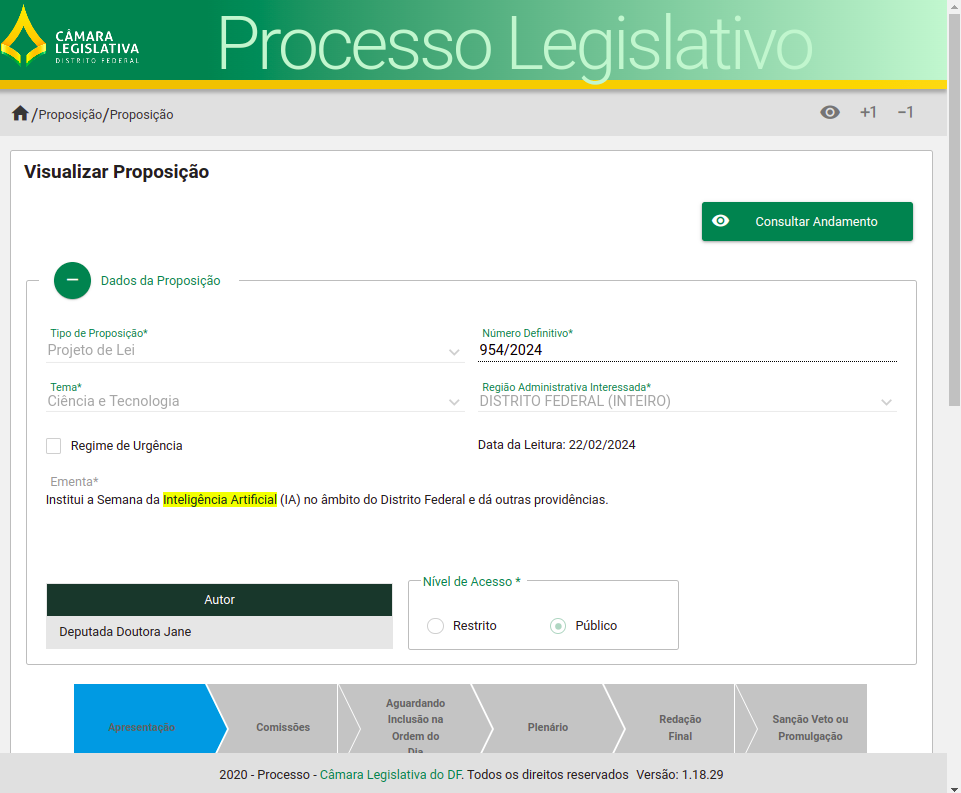
\includegraphics[width=\textwidth]{plePropMetadados.png}
			\caption{Proposal's data}
		\end{subfigure}
	\end{figure}

\end{frame}
%-------------------------------------------------
\begin{frame}
	\frametitle{Methodology}
	\framesubtitle{2 - Data Understanding}	
	\begin{block}{2 - Data Understanding} 
		The dataset contains 22,267 summaries extracted from the Electronic Legislative Process (PLE) system, covering the period from 2021 to May 2024. Each summary is accompanied by its respective thematic classification.
	\end{block}

	\begin{figure}
		
\includegraphics[width=0.2\linewidth]{lupa.png}
	\end{figure}


	% O conjunto de dados contém 22.267 ementas extraídas do sistema de Processo Legislativo Eletrônico (PLE) abrangendo o período de 2021 a maio de 2024. Cada resumo é acompanhado por sua respectiva classificação temática.

\end{frame}
%-------------------------------------------------
\begin{frame}
	\frametitle{Methodology}
	\framesubtitle{3 - Data Preparation}	

	\begin{block}{Data Preparation} 
		\begin{enumerate}

			\item \textbf{Preprocessing}: We discard data classified under ``outro'' and ``não se aplica'' themes. Then, we perform tokenization, normalization, stopword removal, and lemmatization processes.
			
			\item \textbf{Vectorization}:
			\begin{itemize}
				\item \textbf{Multilingual sentence embedding model} based on the MiniLM architecture, a lightweight and efficient BERT variant with 12 transformer layers, to produce high-quality embeddings that capture the semantic meaning of the text. 
				
				\item \textbf{TF-IDF (Term Frequency-Inverse Document Frequency) model} involves converting text into numerical vectors based on the frequency of terms within a document and across a collection of documents. This approach captures the importance of a term in a document relative to the entire dataset.
			\end{itemize}
		\end{enumerate}
	\end{block}
\end{frame}
%-------------------------------------------------
\begin{frame}
	\frametitle{Methodology}
	\framesubtitle{4 - Modeling: Chosen Models - Part I}	
	
	\begin{block}{4 - Modeling} 
		\begin{enumerate}
			\item \textbf{DummyClassifier}: A \textbf{baseline model} that makes predictions using simple rules and establishes a baseline to \textbf{compare the performance of more complex models}.
			
			\item \textbf{Support Vector Machine (SVM)}: A powerful model that \textbf{finds the hyperplane that best separates the classes in the feature space}. It is  effective for high-dimensional spaces and when the number of dimensions exceeds the number of samples.
			
			\item \textbf{Logistic Regression}: A linear model that \textbf{estimates the probability of a binary outcome based on input features}. It is simple and interpretable, good for linearly separable data and understanding feature importance.
		\end{enumerate}
	\end{block}
\end{frame}
% ---------------------
\begin{frame}
	\frametitle{Methodology}
	\framesubtitle{4 - Modeling: Chosen Models - Part II}	
	\begin{block}{4 - Modeling (cont...)} 
		\begin{enumerate}
			\setcounter{enumi}{3}
			\item \textbf{XGBoost (Extreme Gradient Boosting)}: An optimized gradient boosting algorithm that \textbf{builds an ensemble of weak learners (typically decision trees) to improve model performance}. Known for high performance, speed, and scalability.
			
			\item \textbf{Random Forest}: An \textbf{ensemble model that constructs multiple decision trees and aggregates their predictions}. Robust against overfitting, good for handling large datasets with higher dimensionality.
			
			\item \textbf{K-Nearest Neighbors (KNN)}: A \textbf{non-parametric model that classifies a data point based on the majority class of its k nearest neighbors}. Simple and intuitive, effective for small datasets with low noise.
		\end{enumerate}
	\end{block}
\end{frame}
%-------------------------------------------------
\begin{frame}
	\frametitle{Methodology}
	\framesubtitle{4 - Modeling: Justification}	
	\begin{alertblock}{Why Choose These Models?} 
		\begin{enumerate}
			\scriptsize
			\item \textbf{Baseline Comparison}: DummyClassifier provides a benchmark to gauge the performance of more sophisticated models.

			\item \textbf{Linear and Non-Linear Data}: Logistic Regression and SVM cover linear relationships, while Random Forest, XGBoost, and KNN handle non-linear data.

			\item \textbf{Model Performance}: XGBoost and Random Forest are chosen for their strong predictive performance and ability to handle complex datasets.

			\item \textbf{Interpretability}: Logistic Regression is valued for its simplicity and ease of interpretation.

			\item \textbf{Versatility}: SVM, Random Forest, and XGBoost offer versatility across different types of data and problems.

			\item \textbf{Scalability}: XGBoost is particularly chosen for its scalability and efficiency in handling large datasets.




		\end{enumerate}
	\end{alertblock}
\end{frame}



%-------------------------------------------------
\begin{frame}
	\frametitle{Methodology}
	\framesubtitle{5 - Evaluation}	
	
	\begin{block}{5 - Evaluation} 
			Our evaluation metrics include \textbf{Accuracy}, \textbf{Precision}, \textbf{Recall} and \textbf{F1 score}.
	\end{block}

	\begin{block}{} 
		\begin{itemize}
			\item Accuracy is \textbf{straightforward and easy to understand}.
			\item Precision and recall are more informative when dealing with \textbf{imbalanced classes} because they provide insights into the performance of the minority class, which accuracy might overlook.
			
			\item F1 score gives a \textbf{balance between precision and recall as a single metric} to summarize the model performance.
		\end{itemize}
	\end{block}
\end{frame}
%-------------------------------------------------
\begin{frame}
	\frametitle{Methodology}
	\framesubtitle{6 - Deployment}	
	
	\begin{block}{6 - Deployment} 
		\begin{itemize}
			\item The results might be used to create an interface in the PLE system to suggest themes that best fit new proposals.
		\end{itemize}
	\end{block}
\end{frame}
%-------------------------------------------------



% =========================================================
\section{Experimentos Realizados}
\begin{frame}
	\frametitle{Experimentos Realizados}
	
	Falar do Embed
	
	
	
\end{frame}
% =========================================================
\section{Resultados}
\begin{frame}
	\frametitle{Resultados}
	
	
	
	
\end{frame}
% =========================================================
\section{Trabalhos Futuros}
\begin{frame}
	\frametitle{Resultados}
	
	
	
	
\end{frame}
% =========================================================
\section{Conclusões}
\begin{frame}
	\frametitle{Conclusões}
	
	
	
	
\end{frame}
% =========================================================




















